\documentclass[12pt]{article}
\usepackage[utf8]{inputenc}
\usepackage[paperwidth=8.5in, paperheight=180in, margin=1.5in]{geometry}

% removes paragraph indent
\setlength\parindent{0pt}

\usepackage{graphicx}
\usepackage{amsmath}
\numberwithin{equation}{section}
\usepackage{titlesec}
\setcounter{secnumdepth}{4}
\pagenumbering{gobble} % removes page number from TOC and pages

% removes space between enumerate items
\usepackage{enumitem}
\setlist[enumerate]{itemsep=-1ex}

\usepackage{xcolor}
\definecolor{xlinkcolor}{cmyk}{1,1,0,0}
\usepackage[colorlinks,allcolors=xlinkcolor]{hyperref}

% remove dots in TOC
\usepackage[titles]{tocloft}
\renewcommand{\cftdot}{}

\setcounter{tocdepth}{3}

\title{Econometrics}
\author{Andrew Lu}
\date{Mr. Lizardo, Fall 2020}

\begin{document}

    \maketitle
    \label{sec:top}
    \tableofcontents

\section{Introduction to Statistics}

\subsection{Statistical Measures}
\subsubsection{Mean}
\begin{align}
    \mu=\frac{\sum\limits_{i=1}^{N}{x_i}}{N} \\
    \overline{X}=\frac{\sum\limits_{i=1}^{N}{x_i}}{n}
\end{align}

\subsubsection{Variance}
\begin{align}
    \sigma^2=\frac{\sum\limits_{i=1}^{N}{(x_1-\mu)^2}}{N} \\
    s^2=\frac{\sum\limits_{i=1}^{n}{(x_1-\bar{x})^2}}{n-1}
\end{align}
where $\mu$ is the population mean, $\bar{x}$ is the sample mean, $\sigma^2$ is population variance and $s^2$ is sample variance. The denominator is $n-1$ for sample variance calculations because of degrees of freedom.

\subsubsection{Standard Deviation}
\begin{align}
    \sigma=\sqrt{\frac{\sum\limits_{i=1}^{N}{(x_1-\mu)^2}}{N}} \\
    s=\sqrt{\frac{\sum\limits_{i=1}^{n}{(x_1-\bar{x})^2}}{n-1}}
\end{align}

\subsection{Data Distribution}
\subsubsection{Histograms}
\begin{figure}[!ht]
    \centering
    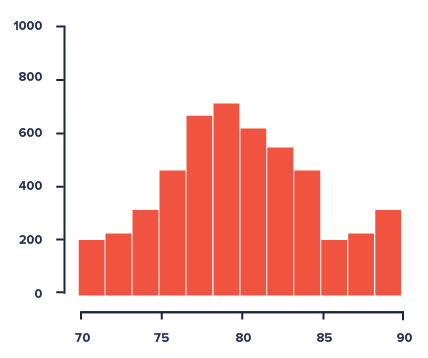
\includegraphics[width=0.6\linewidth]{figures and tables/histogram.png}
\end{figure}

\subsubsection{Box Plots}
\begin{figure}[!ht]
    \centering
    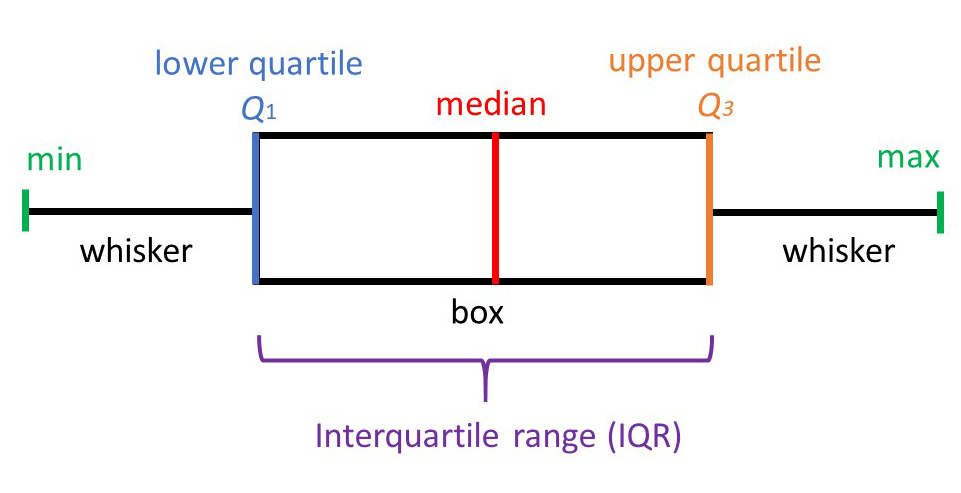
\includegraphics[width=0.8\linewidth]{figures and tables/boxplot.jpg}
\end{figure}
Outliers: any value outside 1.5 $\times$ IQR above Q3 or below Q1
\begin{align}
    IQR = Q3 - Q1
\end{align}

\subsubsection{SOCS}
\begin{enumerate}
    \item Symmetry: positive/right skew, negative/left skew, or normal curve
    \item Outliers: skew the distribution in its direction
    \item Center: mean = balancing point, median = data split in half
    \item Spread: outliers affect spread by impacting skew
\end{enumerate}
\begin{figure}[!ht]
    \centering
    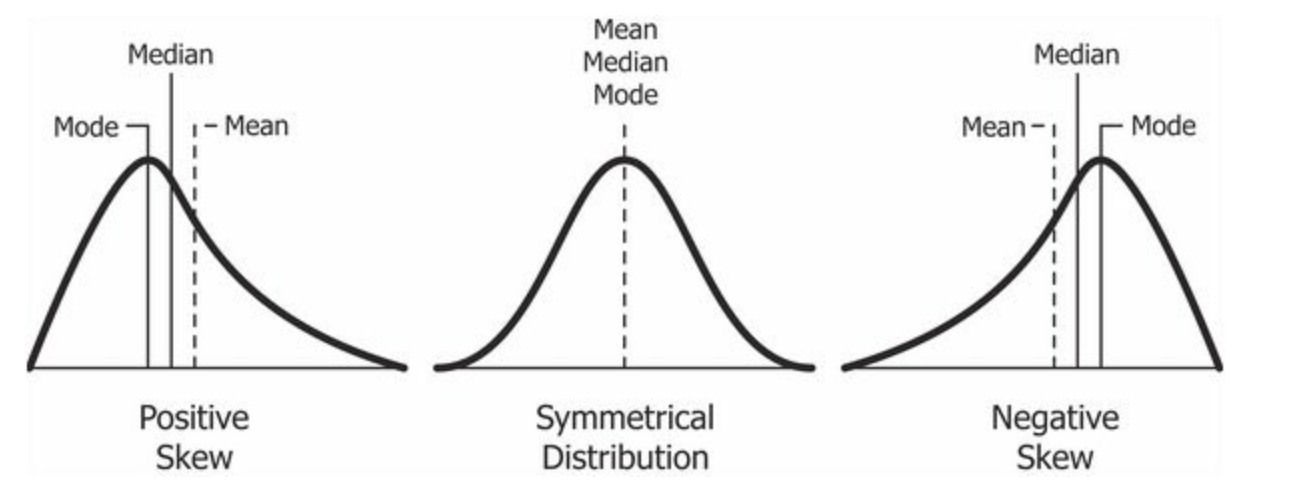
\includegraphics[width=0.9\linewidth]{figures and tables/skew.png}
\end{figure}

\subsection{Probability}
\begin{enumerate}
    \item Conditional Probability:
    \begin{align}
        P(A|B) = \frac{P(A \cap B)}{P(B)}
    \end{align}
\end{enumerate}

\subsection{Discrete Random Variables}
\subsubsection{Measures}
\begin{gather}
    \mu_x = \sum x \times p(x) \\
    \sigma^2_x = (x_1-\mu_x)^2 p_1 + (x_2-\mu_x)^2 p_2 + ... + (x_i-\mu_x)^2 p_i
\end{gather}

\subsubsection{Binomial Situations}
\begin{enumerate}
    \item B: Binary Outcomes
    \item I: Independent Trials
    \item N: Number of Trials
    \item S: Success Probability
\end{enumerate}
\subsubsection{Binomial Probabilities}
\begin{gather}
    \mu_k = np \\
    P(k) = \binom{n}{k} p^k (1-p)^{n-k} \\
    \sigma = \sqrt{np(1-p)}
\end{gather}

\subsection{Continuous Random Variables}
%\subsubsection{Probability Density Function}
%\subsubsection{Area Under Curve (AUC)}
\subsubsection{Normal Distribution}
\begin{figure}[!ht]
    \centering
    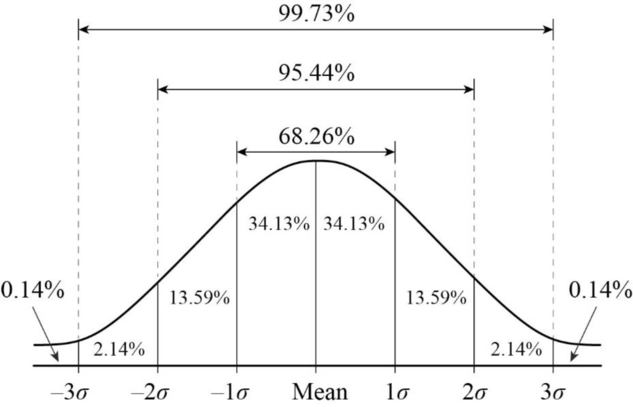
\includegraphics[width=0.8\linewidth]{figures and tables/normalcurve.png}
\end{figure}

\subsubsection{Z-Score}
\begin{gather}
    \text{z-score: } z = \frac{x-\mu}{\sigma}
\end{gather}

\begin{figure}[!ht]
    \centering
    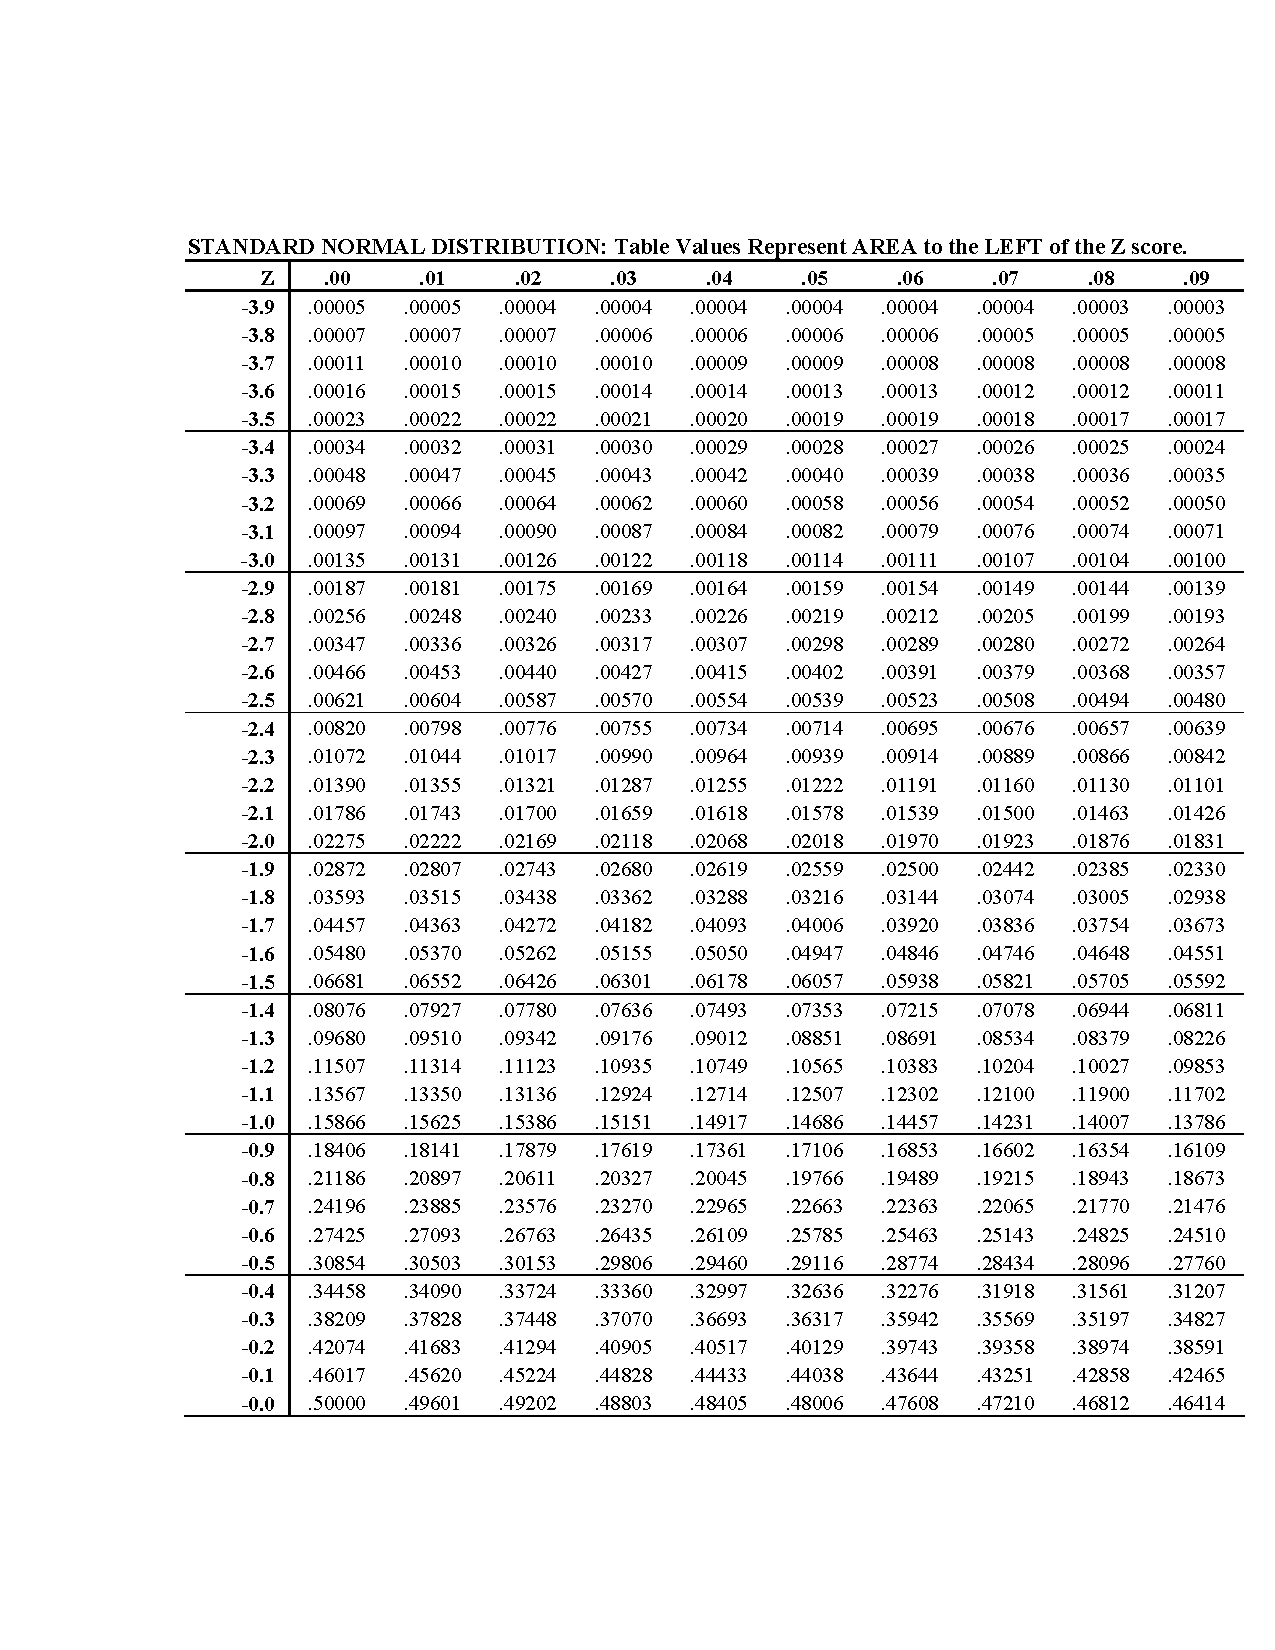
\includegraphics[page=1, width=0.9\linewidth, trim=4cm 4cm 1.25cm 4cm]{figures and tables/standardnormaltable.pdf}
    \label{zscore}
\end{figure}

\begin{figure}[!ht]
    \centering
    \includegraphics[page=2, width=0.9\linewidth, trim=4.1cm 4cm 1.15cm 4cm]{figures and tables/standardnormaltable.pdf}
\end{figure}

\subsection{Sampling Distributions}

\subsubsection{Unknown Variables}
Parameters: measures that describe populations \\
Statistics: measures that describe samples \\
Sampling distribution: distribution of a statistic across all possible samples

\subsubsection{Estimators and Bias}
Estimator: see Section~\ref{sec:confidence_intervals} for definition.
\begin{gather}
    \text{Bias}(W) = \text{E}(W)-\theta \\
    \text{Variability} \propto \frac{1}{\text{sample size}}
\end{gather}
where $W$ is the estimator and $\theta$ is the parameter. \\[0.5cm]
Unbiased estimator: mean of sampling distribution is equal to value of parameter. For example, sample mean is an unbiased estimator because the mean of the sampling distribution of sample means is equal to the value of the parameter.

\subsubsection{Sample Means}
\begin{gather}
    \mu_{\bar{x}}=\mu \\
    \sigma_{\bar{x}}=\frac{\sigma}{\sqrt{n}}
\end{gather}
where $\bar{x}$ is the sampling distribution and $\mu$ is the mean of the population. Thus, sampling distributions have no bias. \\[0.5cm]
Central Limit Theorem: sampling distribution of the mean is approximately normal for any distribution.

\subsection{Confidence Intervals}
\label{sec:confidence_intervals}
\begin{enumerate}
    \item Point estimator: estimate of a population parameter
    \item Point estimate: value of statistic for a sample
    \item Confidence level C: the percent probability that a random sample interval will capture parameter value; in C$\%$ of all samples, the sample interval will include parameter value
    \item Confidence interval: point estimate $\pm$ margin of error; range of plausible values for parameter value
\end{enumerate}

\subsubsection{Margin of Error}
Purpose: addresses sample variability
\begin{gather}
    CI = \bar{x} \pm c_{\alpha/2}*\text{se}(\bar{x}) \\
    \text{se}(\bar{x}) = \frac{s}{\sqrt{n}}
\end{gather}
where $c_{\alpha/2}$ is the critical value (the number of standard errors the interval includes), obtained from the t-table (Figure~\ref{fig:t_table}).

\begin{gather}
    \text{confidence level} \propto CI \\
    CI \propto \frac{1}{\text{sample size}}
\end{gather}
Note: 95\% confident does not mean 95\% chance that true mean is in interval; rather, if data collection was done 100 times, 95 times the interval would contain the true mean. Confidence does not equate to chance.

\subsubsection{t-Table}
\begin{figure}[!ht]
    \centering
    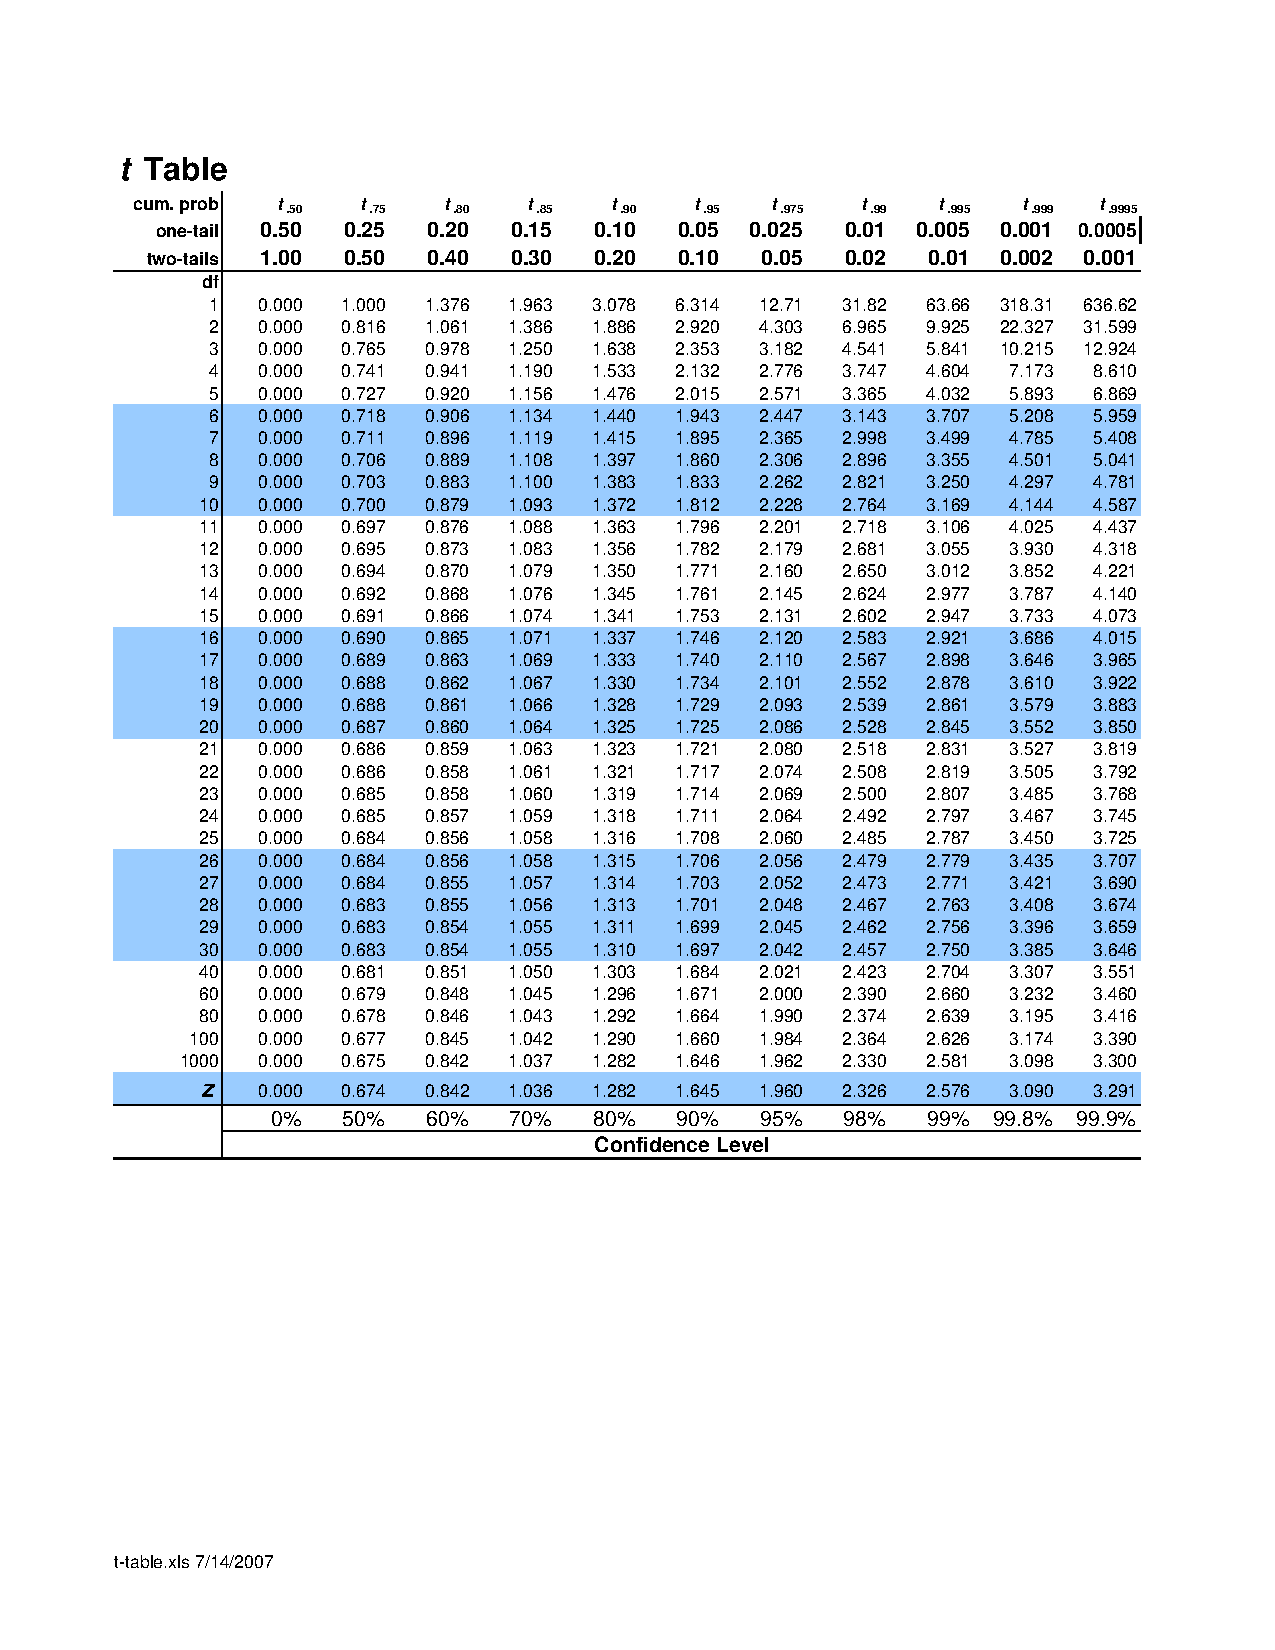
\includegraphics[width=\linewidth, clip, trim=2cm 8cm 2cm 2.5cm]{figures and tables/t-table.pdf}
    \label{fig:t_table}
\end{figure}
\vspace{-1cm}

\subsubsection{Calculation}
Preconditions:
\begin{enumerate}
    \item Random sample selection
    \item $<$10\% of population
    \item Sufficient sample size ($>$30) or normally distributed
\end{enumerate}

Steps:
\begin{enumerate}
    \item Calculate mean
    \item Find margin of error
    \item Find range of sample interval
    \item Interpret in context
\end{enumerate}

\subsection{Hypothesis Testing}

% \subsubsection{Steps}
% \begin{enumerate}
%     \item State hypotheses about population (null, alternative)
%     \item Decide on level of significance
%     \item Compare sample analysis with hypothetical
% \end{enumerate}

\subsubsection{Hypotheses}
Null hypothesis: hypothesis assumed to be true (specific value)
\begin{gather}
    \text{H}_0 : \theta = .80
\end{gather}
where $\theta$ is the parameter being analyzed. \\[0.5cm]
Alternative hypotheses (one-sided or two-sided):
\begin{gather}
    \text{H}_1 : \theta < .80 \\
    \text{OR} \\
    \text{H}_1 : \theta \neq .80
\end{gather}

\subsubsection{Analytical Errors}
\begin{enumerate}
    \item Type I error: rejecting H$_0$ when actually true
    \item Type II error: failing to reject H$_0$ when actually false
\end{enumerate}

\subsubsection{Significance Level}
\begin{gather}
    \alpha = P(\text{Reject H}_0|\text{H}_0)
\end{gather}
where $\alpha$ is the probability of type I error. $\alpha$ is typically 0.05.

\subsubsection{p-values}
p-value: the largest significance level given sample while still failing to reject the null. In other words, likelihood of another sample having the t-statistic equal or larger assuming null hypothesis.

\subsubsection{Calculation}
\begin{enumerate}
    \item Confirm preconditions (random, sample size $>$ 30, sample size $<$ 10\% or normally distributed)
    \item Calculate t statistic $T$ (see Equation~\ref{eq:t})
    \item Find critical value $c$ based on target significance level (see \href{fig:t_table}{t-table}), or find p-value from $T$ (see \href{sec:appendix}{Appendix} for \verb|TDIST|, primarily two-tailed)
    \item Compare $T$ and $c$, or p-value and target significance level, to determine whether to reject H$_0$
\end{enumerate}
\begin{gather}
    T = \frac{\bar{x}-\mu_0}{\frac{s}{\sqrt{n}}} \label{eq:t}
\end{gather}

\subsubsection{Example}
Context: $\bar{x}$ = 520g, $s$ = 75g, n = 25, $\alpha$ = 0.05 \\
H$_0$ : $\mu$ = 500g
\begin{align}
    T &= \frac{\bar{x}-\mu_0}{\frac{s}{\sqrt{n}}} \\
    &= \frac{520-500}{\frac{75}{\sqrt{25}}} = \frac{20}{15} = 1.33 \\
    c &= 1.711 \text{ (from t-table t$_{0.95}$, df = 24)}
\end{align}
The calculation found that $T<c$. Thus, there is not sufficient evidence to reject the null hypothesis.
\subsubsection{Power of a Test}
\begin{gather}
    \pi(\theta) = P(\text{Reject H}_0|\theta) = 1 - P(\text{Type II}|\theta)
\end{gather}
where $\pi$ is the probability of rejecting a false null.

\subsection{Basic Regressions}

% \subsubsection{Correlation Coefficient}
% R: \{-1,1\}

\subsubsection{Simple Regression Model}
\begin{gather}
    y = \beta_0 + \beta_1 x + u
\end{gather}
where $\beta_1$ is the slope parameter, $\beta_0$ is the intercept, and $u$ is the unobserved error.

\subsubsection{Background}
\begin{gather}
    e = \hat{u} = y - \hat{y}
\end{gather}
where $e$ and $\hat{u}$ is the residual, $y$ is the actual value, and $\hat{y}$ is the predicted value. \\[0.5cm]

Zero conditional mean assumption: independent variable does not affect or provide any information about unobserved factors.
\begin{gather}
    E(u|x) = 0 \label{eq:zero_conditional_mean} \\
    E(y|x) = \beta_0 + \beta_1 x
\end{gather}

\subsubsection{OLS Calculation}
\begin{gather}
    \hat{\beta}_0 = \bar{y} - \hat{\beta}_1 \bar{x} \\
    \bar{\beta}_1 = \frac{\sum\limits_{i=1}^{n} (x_i-\bar{x})(y_i-\bar{y})}{\sum\limits_{i=1}^{n} (x_i-\bar{x})^2}
\end{gather}
where $\hat{\beta_0}$ is the predicted y-intercept and $\hat{\beta_1}$ is the predicted slope based on ordinary least squares regression. $SST$ is sum of squares total, $SSE$ is sum of squares error, and $SSR$ is sum of squares regression.

\subsubsection{Key Properties}
\label{sec:key_properties}
\begin{align}
    1.& \sum_{i=1}^{n} \hat{u}_i = 0 \\
    2.& \sum_{i=1}^{n} x_i \hat{u}_1 = 0 \\
    3.&\, (\bar{x},\bar{y}) \text{ on regression line}
\end{align}
where $\hat{u}_i$ is the residual of data point $i$.

\subsubsection{Goodness of Fit}
\label{sec:goodness_of_fit}
\begin{gather}
    SST = \sum_{i=1}^{n} (y_i-\bar{y})^2 \\
    SSE = \sum_{i=1}^{n} (\hat{y}_i-\bar{y})^2 \\
    SSR = \sum_{i=1}^{n} \hat{u}_i^2 = \sum_{i=1}^{n} (y_i-\hat{y}_i)^2 \\
    SST = SSE + SSR \\
    R^2 = \frac{SSE}{SST} = 1 - \frac{SSR}{SST}
\end{gather}
where $R^2$ is the coefficient of determination and a larger $R^2$ indicates the regression explains variation well.

\begin{gather}
    \bar{R}^2 = 1 - \frac{SSR/(n-k-1)}{SST/(n-1)}
\end{gather}
where $\bar{R}^2$ is the adjusted $R^2$ and $k$ is the number of independent variables in regression. Typically adjusted $R^2$ is used for non-nested models (where removing independent variables from one of the regressions can make the other regression have the same set of independent variables).

\section{Multivariate Regressions on Cross-Sectional Data}

\subsection{OLS Regressions Basics}
Begin use of Gretl software \\[0.5cm]
A linear regression is any equation that follows a linear pattern between two variables or any modified version of two variables (logs, exponents, etc) \\[0.5cm]
Note: for log dependent variables with large coefficients for independent variables, use $100 [e^{\beta}-1]\%$ instead.

\subsubsection{Gauss-Markov Assumptions for Simple Linear Regressions}
\begin{enumerate}
    \item SLR.1: Functional form $y = \beta_0 + \beta_1 x + u$
    \item SLR.2: Random sample
    \item SLR.3: Explanatory variable must vary ($\sigma \neq 0$)
    \item SLR.4: Zero conditional mean (see Equation~\ref{eq:zero_conditional_mean})
    \item SLR.5: Homoskedasticity ($Var(u|x) = \sigma^2$ (constant))
\end{enumerate}
$\qquad \Rightarrow E(\hat{\beta}_0) = \beta_0, E(\hat{\beta}_1) = \beta_1$

\subsubsection{Sampling Variance of OLS Estimators}
\begin{gather}
    Var(\hat{B}_1) = \frac{\sigma^2}{\sum_{i=1}^{n} (x_i - \bar{x})^2} = \frac{\sigma^2}{SST_x} \\
    Var(\hat{B}_0) = \frac{\sigma^2 n^{-1} \sigma^2}{SST_x} = \frac{\sum_{i=1}^{n} {x_i^2}}{SST_x}
\end{gather}
As $\sigma$ increases, $Var(\hat{B}_1)$ increases. As range increases, $SST_x$ increases and $Var(\hat{B}_1)$ decreases.

\begin{gather}
    \hat{\sigma}^2 = \frac{1}{n-2} \sum_{i=1}^{n} \hat{u}_i^2 \\
    \text{se}(\hat{B}_1) = \frac{\hat{\sigma}}{\sqrt{SST_x}}
\end{gather}
where $\hat{\sigma}$ is the standard error of the regression, or the standard deviation of the error.

\subsection{Multiple Linear Regression Model}
\begin{gather}
    y = \beta_0 + \beta_1 x_1 + \beta_2 x_2 + ... + \beta_k x_k + u
\end{gather}

\subsubsection{Commonalities with Simple Regression}
\begin{enumerate}
    \item See \ref{sec:key_properties}, applicable for each variable
    \item See \ref{sec:goodness_of_fit}
\end{enumerate}

\subsubsection{MLR Assumptions}
\begin{enumerate}
    \item MLR.1: Functional form
    \item MLR.2: Random sample
    \item MLR.3: No perfect collinearity (SLR.3 plus no perfect linearity between two independent variables)
    \item MLR.4: Zero conditional mean
    \item MLR.5: Homoskedasticity
    \item MLR.6: Normality of error
\end{enumerate}
$\qquad \Rightarrow E(\hat{\beta}_j) = \beta_j, j = 0, 1, ..., k$

\subsubsection{Omitted Variable Bias}
Given $y = \beta_0 + \beta_1 x_1 + \beta_2 x_2 + u$, if $x_2$ is excluded, $\tilde{y} = \tilde{\beta}_0 + \tilde{\beta}_1 x_1$.
\begin{gather}
    \tilde{\beta}_1 = \hat{\beta}_1 + \hat{\beta}_2 \tilde{\delta}_1 \\
    E(\tilde{\beta}_1) = \beta_1 + \beta_2 \tilde{\delta}_1 \\
    \text{Bias}(\tilde{\beta}_1) = E(\tilde{\beta}_1) - \beta_1 = \beta_2 \tilde{\delta}_1
\end{gather}
where $\tilde{\delta}_1$ is the slope of the regression of $x_2$ on $x_1$.

\subsubsection{Variance}
\begin{gather}
    Var(\hat{B}_j) = \frac{\sigma^2}{SST_j(1-R_j^2)}
\end{gather}
where $R_j^2$ is the $R^2$ from regressing $x_j$ on the other independent variables.\\[0.5cm]
Multicollinearity leads to high variance as seen by a larger $R_j^2$. Removing a variable leads to larger bias.

\begin{gather}
    VIF_j = \frac{1}{1-R_j^2}
\end{gather}
where $VIF_j$ is the variable inflation factor for $x_j$. Typically $VIF$ should be below 10.

\begin{gather}
    \hat{\sigma}^2 = \frac{1}{n-k-1} \sum_{i=1}^{n} \hat{u}_i^2
\end{gather}
where $k$ is the number of independent variables in regression.

\begin{gather}
    se(\hat{B}_j) = \sqrt{\frac{\hat{\sigma}^2}{SST_j(1-R_j^2)}}
\end{gather}
Note that the equation includes $\hat{\sigma}$, not $\sigma$. $sd(\hat{B}_j)$ uses $\sigma$.

\subsection{Inference}

\subsubsection{T-statistic}
\begin{gather}
    T = \frac{\hat{B}_j}{se(\hat{B}_j)} \\
    df = n-k-1
\end{gather}

\subsubsection{p-value}
Probability of coefficient value assuming null hypothesis (using gretl)

\subsubsection{F-test}
Joint significance: see which variables do not affect explanatory power of regression \\[0.5cm]
Compute $SSR$ for restricted and unrestricted models to find F-statistic:
\begin{align}
    F &= \frac{(SSR_r - SSR_{ur})/q}{SSR_{ur}/(n-k-1)} \\
    &= \frac{(R_{ur}^2 - R_{r}^2)/q}{(1-R_{ur}^2)/(n-k-1)}
\end{align}
where $q$ is the number of restricted variables. Use gretl to find p-value.

% \begin{gather}
%     H_0 : \beta_3 = 0, \beta_4 = 0, \beta_5 = 0
% \end{gather}

\subsection{Dummy Variables}
Dummy variables: a qualitative characteristic that takes a value of 0 or 1 as a variable (e.g., $female$ in $wage = \beta_0 + \delta_0  female + \beta_1 educ + u$) \\[0.5cm]
Note: do not include all categories of the qualitative characteristic in the regression

\subsubsection{Interaction}
Interaction variable: additional variable that allows test of whether one variable's effects vary based on grouping (e.g., $female \cdot educ$)

\subsubsection{Differences across Groups}
Create unrestricted model with interaction variables for all variables and run test of joint significance (F-test) or run Chow test without interaction variables (separate regressions for different groups)

\subsubsection{Chow Test}
\begin{gather}
    F = \frac{SSR_p - (SSR_1 + SSR_2)}{SSR_1 + SSR_2} \frac{n - 2(k+1)}{k+1}
\end{gather}
where $n$ is number of observations and $k$ is the number of interactions.

\subsubsection{Linear Probability Model}
Determines probability of binary variable being true by using a continuous variable \\[0.5cm]
Note: linear probability models are heteroskedastic

\subsection{Heteroskedasticity}

Potential issues: variance formulas invalid \\
Nonissues: still no bias, $R^2$ unchanged, still can use gretl (with robust error enabled)

\subsubsection{Heteroskedasticity-Robust Standard Errors}
\begin{gather}
    \widehat{Var}(\hat{\beta}_j) = \frac{\sum_{i=1}^{n} \hat{r}_{ij}^{2} \hat{u}_i^2}{SSR_j^2}
\end{gather}
where $\hat{r}_{ij}^{2}$ is the residual of the $i$th value regressing $x_j$ on all other independent variables and $SSR_j^2$ is the $SSR$ of $x_j$ on all other independent variables.

\subsubsection{Testing for Heteroskedasticity}
Hypothesis test:
\begin{gather}
    H_0 : Var(u|x) = E(u^2) = \sigma^2
\end{gather}

Breusch-Pagan test: assumes no linear relationship between $u^2$ and independent variables to find p-value (use gretl)
\begin{gather}
    u^2 = \delta_0 + \delta_1 x_1 + \delta_2 x_2 + ... \\
    H_0 : \delta_1 = \delta_2 = ... = 0
\end{gather}

White test: assumes $u^2$ uncorrelated with independent variables, their squares, or their cross products \\[0.5cm]
Alternative White test: assumes no linear relationship between $u^2$ and fitted values and fitted values squared

\subsubsection{Weighted Least Squares}
In order to run weighted least squares in gretl, define an independent variable as 1/(fitted values) and use the variable as the weight.

\subsection{Functional Form Misspecification}
Functional form misspecification: not specifying higher order or log forms may lead to high bias

\subsubsection{Ramsey RESET Test}
RESET (Regression Equation Specification Error Test) Test: include squares and higher order fitted values to regression to determine whether to reject null hypothesis of properly specified regression.

\section{Multivariate Regression on Time Series Data}

The basics:
\begin{enumerate}
    \item Temporally ordered
    \item Sequences of random variables (stochastic process)
    \item Sample itself is one random path for time series out of many possible paths
\end{enumerate}

\subsection{Time Series Models}

\subsubsection{Static Models}
Contemporaneous relationship between variable (e.g., Phillips Curve tradeoff between inflation and unemployment)

\begin{gather}
    y_t = \alpha_0 + \delta_0 z_t
\end{gather}

\subsubsection{Finite Distributed Lag (FDL) Model}
Model with variables for lagged effects (one-time shock or permanent shock)
\begin{gather}
    y_t = \alpha_0 + \delta_0 z_{t} + \delta_1 z_{t-1} + \delta_q z_{t-q} + u_t
\end{gather}
where $\delta_{s}$ is the coefficient of the effect from a shock $t-s$ years ago based on independent variable $z_{t-s}$.

\subsubsection{Time Series Assumptions}
\begin{enumerate}
    \item TS.1: Linear regression
    \item TS.2: No perfect collinearity
    \item TS.3: Zero conditional mean for all time periods
    \item TS.4: Homoskedasticity
    \item TS.5: No serial correlation/autocorrelation (errors across time periods)
    \item TS.6: Normality (normally distributed errors)
\end{enumerate}

\subsection{Trending Time Series}

\subsubsection{Linear and Exponential Time Trend}
\begin{gather}
    y_t = \alpha_0 + \alpha_1 t + e_t \\
    \log(y_t) = \alpha_0 + \alpha_1 t + e_t
\end{gather}

Detrend: include time trend to evaluate non-trended effects of independent variables

\subsection{Stationary and Weakly Dependent Time Series}

Stationary Stochastic Process: probability distribution constant
Covariance Stationary Process: constant $x_t$, constant variance for $x_t$, and covariance $x_t$ and $x_{t+h}$ is only affected by $h$, not $t$

Weak Dependence: some correlation between $x_t$ and $x_{t+h}$ but decreases as $h$ increases, allows for OLS (e.g., moving average models, autoregressive models)

\subsubsection{Weaker Assumptions}
\begin{enumerate}
    \item TS.1: Linear regression and weakly dependent
    \item TS.2: No perfect collinearity
    \item TS.3: Contemporaneously exogenous independent variables
    \item TS.4: Contemporaneously homoskedastic
    \item TS.5: No autocorrelation
\end{enumerate}

\subsection{Highly Persistent Time Series}

\begin{gather}
    y_t = y_{t-1} + e_t
\end{gather}

\subsubsection{Addressing Autocorrelation}
Use differencing ($\Delta$) when autocorrelation is high \\[0.5cm]
Autocorrelation shortcomings: standard errors (and thus t-tests and F-tests) invalid, no longer minimum variance estimator \\[0.5cm]
Tests for autocorrelation:
\begin{enumerate}
    \item tests on residuals from lagged residuals (strictly exogenous)
    \item Durbin-Watson test (strictly exogenous): $\frac{\sum\limits_{t=2}^{n}(\hat{u}_{t}-\hat{u}_{t-1})^2}{\sum\limits_{t=1}^{n}\hat{u}_t^2}$ ($<$2 positive autocorrelation, $>$2 negative autocorrelation)
    \item tests on residuals and lagged residuals and independent variables (not strictly exogenous)
    \item Breusch-Godfrey test of residuals on lagged residuals, independent variables, all relevant lags
\end{enumerate}

Correcting for autocorrelation:
\begin{enumerate}
    \item Respecify model (e.g., Cochrane-Orcutt, Prais-Winston)
    \item Autocorrelation robust standard errors
\end{enumerate}

\subsection{Financial Econometrics}

\subsubsection{Capital Asset Pricing Model (CAPM)}
Risk: unsystematic/diversifiable (risk of a specific asset), systematic (market risk) \\
CAPM assumptions: rational investors, no diversifiable risk, risk free alternatives, maximize expected return at given systematic risk \\
Risk-return tradeoff: expected return only increases when risk increases \\

Efficient frontier, capital asset line (CAL)
\begin{gather}
    E(R_i) = R_F + \beta_i [E(R_M)-R_F] \\
    \beta_i = \frac{cov(R_i,R_M)}{\sigma^2(R_M)}
\end{gather}
where $R_F$ is risk-free return, $R_M$ is market return, $R_i$ is expected return for a risk level of $i$.

\section{Appendix}
\label{sec:appendix}

\begin{table}[!ht]
    \centering
    \footnotesize
    \begin{tabular}{c|c c}
        Function                &   Inputs  &   Output \\ \hline
        \verb|NORMDIST|$^1$     &   value on dist, mean, std deviation, cumulative  & probability   \\
        \verb|NORMINV|          &   probability, mean, std deviation            &   value at prob \\
        \verb|BINOMDIST|$^2$    &   successes, total, probability per trial, cumulative   &   probability \\
        \verb|T.INV|            &   one-tailed probability, degrees of freedom  &   critical value \\
        \verb|T.INV.2T|         &   two-tailed probability, degrees of freedom  &   critical value \\
        \verb|TDIST|            &   critical value or T, deg of freedom, 1 or 2 tail    &  probability (p) \\
        \verb|CONFIDENCE.T|     &   1.00 - confidence level, std dev, sample size    &   half CI width \\
    \end{tabular}
    \label{tab:sheet_functions}
    \caption{Google Sheet Functions}
\end{table}
\footnotesize{$^1$cumulative = true, $^2$cumulative = false (in most cases)}

% \section{Other}
% \begin{enumerate}
%     \item reduce space between enumerate items [done]
% \end{enumerate}

\normalsize
\begin{flushright} \hyperref[sec:top]{back to top} \end{flushright}
\end{document}